\section{\acl{LSTM}}
\textit{Daniel Andrés López, Frank Reichwein}

Eine weitere Art eine Klassifizierung vorzunehmen ist es ein neuronales Netz zu
verwenden. Dieser Ansatz ist durch die Biologie motiviert und lehnt sich an die
Arbeitsweise eines Gehirns an. Im Gehirn sind Neuronen über Synapsen iteinander
verbunden. Nervenbahnen aus dem gesamten Körper erreichen die Neuronen und
stimulieren sie in unterschiedlicher Intensität. Wird dabei ein Schwellwert
überschritten ist dieses Neuron aktiviert und sendet ebenfalls einen Impuls an
die mit ihm über die Synapsen verbundenen Neuronen. Dies geschieht fortlaufend.
Die Synapsen sind jedoch unterschiedlich stark ausgeprägt, um auch eine
unterschiedliche Stimulierungsintensität weiterzugeben. Dies kommt einer
Gewichtung der Neuronen gleich, da die Eingangssignale einen unterschiedlich
starken Einfluss auf das stimulierte Neuron haben. Die Synapsen sind jedoch
nicht fest und von vornerein vorgegeben. Sie werden kontinuerlich auf- und
abgebaut bzw. verändert. Dieser Vorgang wird im Allgemeinen Lernen bezeichnet.
Die erlebten Erfahrungen werden in dem Netz von Neuronen und Synapsen
verarbeitet und dadurch gespeichert. Erreichen das Gehirn nun neue
Sinneseindrücke werden die Neuronen erneut stimuliert und je nach Ergebnis
werden bestimmte Erinnerungen, Gefühle, Aktionen oder anderes erlebt und
ausgeführt. Jedoch sind sie nicht direkt an ein bestimmtes Ereignis geknüpft,
sondern wurden durch verschiedene Erfahrungen verallgemeinert, um so
verschiedenen Situationen gut verarbeiten zu können. 

\paragraph{Modelle von Neuronen und Synapsen}
Im Bereich des maschinellen Lernen wird versucht die Funktionsweise eines
Gehirns bzw. Netzes aus Neuronen und Synapsen nachzubilden. Dies wird durch
vereinfachte Modelle von Neuronen und Synapsen erreicht. Ein einfaches Modell
wird hier als Grundlage verwendet. Es ist das Modell von McCulloch und Pitts von
1943 (vgl. \cite{Mcc43}) und modelliert ein Neuron mit $n$-vielen Eingabewerten
($x_1,\ldots,x_n$) und einem Ausgabewert $y$. Die Eingabewerte entsprechen der
Aktivierung eines Vorgängerneurons und der Ausgabewert der Aktivierung des
betrachteten Neurons.
\textbf{TODO Picture McCulloch and Pitts Neuron} Die \autoref{} zeigt den Aufbau
eines solchen Neurons. Die Eingaben weren dabei zuerst im \textit{Addierer}
summiert, eine Schwellwertfunktion (bzw. allgemeiner eine Aktivierungsfunktion)
bestimmt dann mit der Summe den Ausgabewert (die Aktivierung) des Neurons. Des
Weiteren werden auch die Synapsen nachgebildet in dem jeder Eingabewert bei der
Summierung individuell gewichtet wird. Die Gewichte entsprechen den
unterschiedlich stark ausgeprägten Synapsen. Das klassische Modell erlaubt nur
binäre Ein- und Ausgaben, dies kann jedoch auf reelle Zahlen erweitert werden,
um unterschiedlich starke Stimulierungen bzw. auch negative Werte (Hemmungen)
zuzulassen.

\paragraph{Neuronale Netzwerke}
Einzelne Neuronen können allerdings kein Gehrin nachbilden. Aus diesem Grund ist
die Kombination mehrerer Neuronen zu einem neuronalen Netz nötig. Im einfachsten
Fall entsteht dabei ein \textit{Perzeptron} (vgl.
\cite{rosenblatt58a,1165576}). Es werden $n$-viele Neuronen
verwendet. Alle Eingaben werden von allen Neuronen verarbeitet und jedes Neuron
hat eine eigene Aktivierung. Die Gewichte (Synapsen) sind individuell für jedes
Neuron. Die Ausgaben ergeben den Ausgabevektor $\bf{y}$ des Netzwerkes. Um
komplexere Sachverhalte darstellen zu können, ist es nötig Neuronen in Abhängigkeit
voneinander zu betrachten. Dies wird in \acp{MLP} vorgenommen \cite{1165576}.
Mehrere Perzeptrons werden hintereinandergeschaltet, sodass die Ausgabe des
einen Perzeptrons (ein Layer) die Eingabe des nächsten Perzeptrons ist.
Lediglich die Ausgabe des letzten Perzeptrons ist die Ausgabe des Netzwerks.
Ein Netzwerk kann als gerichteter Graph dargestellt werden. Die Richtung
entspricht dem Datenfluss. Perzeptrons und \acp{MLP} sind azyklische Graphen,
d.h. die Verbindungen von Neuronen gehen nur in Vorwärtsrichtung und bilden
somit keinen Kreis. Daher werden diese Netzwerke \textit{Feedforward}-Netzwerke
genannt. Um besser die Funktionsweise von Gehirnen nachzubilden ist es notwendig
auch Verbidnungen von Neuronen auf sich selbst zuzulassen. Somit entsteht ein
zyklischer Graph und das Netzwerk wird zu einem Rekurrenten Neuronalen Netz
(\acsu{RNN}).
\textbf{TODO Bilder von Neuronalen Netzen zur Verdeutlichung}

Im Rahmen dieses Kpaitel wird erläutert, wie \acsp{LSTM}, eine spezielle Form
von \acp{RNN}, zur Klassifikation von Gesten des schallbasierten Dopplereffekts
genutzt werden können. Dazu wird zuerst darauf eingegangen wie ein \ac{LSTM} im
Allgemeinen funktioniert und wie ein solches Netzwerk trainiert werden kann.
Darauf aufbauend wird das Verfahren auf das Projekt angepasst. Es werden die
Datenaufbereitung, die Anpassung des Klassifikators, die Implementierung in
Python, das Training und eine Evaluierung besprochen.


\subsection{Funktionsweise des Klassifikators (Allgemein)}

Ein \acl{LSTM} ist ein spezielles \ac{RNN}. Es wurde 1997
vorgestellt\cite{Hochreiter:1997}. Wie allgemein Neuronale Netze und
insbesondere \ac{RNN} können auch \ac{LSTM}-Netze biologisch motiviert werden.
Neuronen im Gehirn verhalten sich nicht mit der gleichen Eingabe gleich.
Vielmehr reagieren sie abhängig von verschiedenen Situationen anders. Beinflusst
wird dies durch vorangegangene Ereignisse. Eindrücke (Eingaben) werden so in
einen zeitlichen Bezug gestellt und dadurch entsteht eine zusammenhängende
Erinnerung. Diese wird wie eine einzelne Eingabe ebenfalls generalisiert in den
Synapsen und Neuronen gespeichert. Mit Hilfe der \ac{LSTM} Architektur wird
versucht dieses Verhalten nachzuahmen. 

In einem Netz mit \ac{LSTM}-Einheiten sind diese keine einzelnen Neuronen
sondern Blöcke aus mehreren Neuronen und Toren (ein Tor bzw. engl.
Gate bestimmt ob ein anliegender Wert weitergegeben wird oder nicht).
Die Blöcke werden im Netz wie ein Neuron behandelt. Sie erhalten alle Eingaben
und geben einen Wert aus. \ac{LSTM}-Layer werden in der Regel als Hidden-Layer
in einer \ac{MLP}-Architektur eingesetzt, jedoch ist kein weiteres Hidden-Layer
nötig. Für das Ausgabe-Layer werden je nach Problemstellung unterschiedliche
Arten verwendet, z.B. lineare, sigmoidale oder Softmax-Layer.

\paragraph{\ac{LSTM}-Block}

\begin{figure*}[htfp]
	\begin{center}
	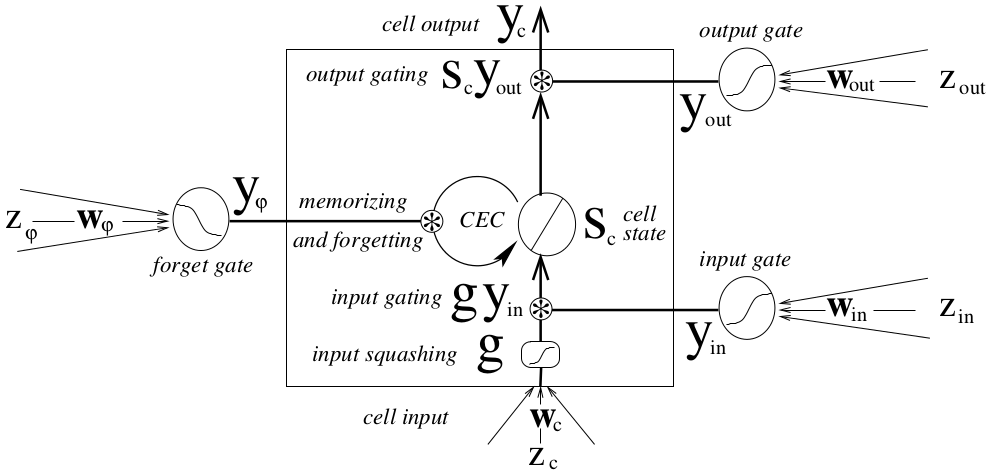
\includegraphics[width=0.8\textwidth]{lstm/lstm_block_formulas}
	\caption[\acs{LSTM} Block]{\acs{LSTM} Block mit einer Memoryzelle ohne
	Peepholes} \tiny Quelle: \cite{Gers2002b}
	\label{fig:lstm_block}
	\end{center}
\end{figure*}  

\autoref{fig:lstm_block} zeigt den schematischen Aufbau eines \ac{LSTM}-Blocks
nach \cite{Gers2002b}. Der Block besteht dabei aus mehreren Komponenten. Dese
werden anhand ihrer Berechnung bei einem \textit{vorwärts} Durchlauf der Daten
erläutert.
\begin{itemize}
	\item Eingabewerte $y_m(t-1)$
	\item Zelleingang $z_c$ berechnet durch \autoref{eq_lstm_in}
	\item Inputgate $z_{in}$ berechnet nach \autoref{eq_lstm_gate}
	\item Forgetgate $z_\varphi$ berechnet durch \autoref{eq_lstm_gate}
	\item Memoryzelle mit dem aktuellen Wert $s_c$ berechnet durch
	\autoref{eq_lstm_cs}
	\item Outputgate $z_{out}$ berechnet nach \autoref{eq_lstm_gate}
	\item Ausgabewert $y_m(t)$ berechnet durch \autoref{eq_lstm_out}
\end{itemize}

% Inputs
\begin{equation}
\label{eq_lstm_in}
z_{c}(t) = \sum \limits_{m} w_{c,m}y_m(t-1)
\end{equation}

% Gate Allgemein
\begin{equation}
\label{eq_lstm_gate}
\begin{split}
y_{gate}(t) &= f_{gate}(z_{gate}(t))\\
z_{gate}(t) &= \sum \limits_{m} w_{gate,m}y_m(t-1)
\end{split}
\end{equation}

% Cell State
\begin{equation}
\label{eq_lstm_cs}
\begin{split}
s_{c}(0) &= 0\\
s_{c}(t) &= y_{\varphi}(t)s_{c}(t-1) +
y_{in}(t)g(z_{c}(t))
\end{split}
\end{equation}

% Output
\begin{equation}
\label{eq_lstm_out}
\begin{split}
y_{c}(t) &= y_{out}(t)s_{c}(t)\\
\end{split}
\end{equation}

Die Funktionen $f_{in}$, $f_{\varphi}$ und $f_{out}$ sind sigmoidale Squashing
Funktionen, die Eingabewerte an den Gates auf $y\approx1$ oder $y\approx0$
zusammenfassen. Dies hat zur Folge, dass an den \textit{gating} Stellen Werte
gelöscht (bei $y\approx0$) oder unverändert durchgelassen werden (bei
$y\approx1$). Somit kontrolliert das Inputgate (\autoref{eq_lstm_cs} zweiter
Teil, zweiter Summand), ob neue Werte die Memoryzelle erreichen, das Forgetgate
(\autoref{eq_lstm_cs} zweiter Teil vorne), ob der vorherige Zustand erhalten
bleibt oder nicht berücksichtigt wird und das Outputgate (\autoref{eq_lstm_out})
wann ein Zustand der Memoryzelle ausgegeben wird. Grundsätzlich hat jeder
Eingang in den \ac{LSTM}-Block inklusive der Eingänge der Gates ein eigenes
Gewicht. Diese sind mit $w_{i,m}$ benannt, wobei $i$ der Eingang oder das Gate
repräsentiert und $m$ der index über die Eingabeimension ist. Daher hat ein
\ac{LSTM}-Block $4\cdot Eingabedimension$ viele Gewichte. 

\acp{LSTM} werden durch ihre autorekurrente Verbindung der Memoryzelle zu
\acp{RNN}. Diese rekurrente Verbindung ist besonders, da sie beim Training
Fehler nicht vor in die komplette Vergangenheit zurückpropagiert. Erreicht wird
das durch ein Gewicht der Verbindung von $1.0$ (\autoref{eq_lstm_sc}). Das zuvor
beschriebene Forgetgate nimmt Einfluss auf dieses Gewicht. Soll der Wert
$s_c(t-1)$ in der Brechnung nicht berücksichtigt werden, setzt das Gate das
Gewicht auf $\approx0$ andernfalls behält es den aktuellen Wert des gewichts mit
$\approx1$ bei. 

Eine Erweiterung zu dem vorgestellten \ac{LSTM}-Block sind zusätzlich weitere
rekurrente Verbindungen (vgl. \cite{Gers2002b}). Diese weiteren rekurrenten
Verbindungen werden \textit{Peepholes} genannt und verbinden die die Memoryzelle
zusätzlich zu den Gates, sodass sich die \autoref{eq_lstm_gate} für die Gateaktivierung
wie folgt ändert:
% Gate Allgemein
\begin{equation}
\label{eq_lstm_gate_peephole}
\begin{split}
z_{gate}(t) &= \sum \limits_{m} w_{gate,m}y_m(t-1) \\
			&+ w_{gate,c} s_c(t-1)
\end{split}
\end{equation}

$w_{gate,c}$ ist dabei das Gewicht der rekurrenten Verbindung von der
Memoryzelle zum Gate. Peepholeverbinsung machen auf diese Art die Information
der Memoryzelle den Gates verfügbar und können so das Netzwerk verbessern
\cite{Gers2002b}. 

Der beschriebene \ac{LSTM}-Block enthält eine einzelne Memoryzelle. Denkbar sind
jedoch Blöcke mit mehreren Memoryzellen, die sich dann die die drei Gates
teilen. Auch sind hier Peepholeverbinsungen möglich, die Gates berücksichtigen
dann alle Werte der Memoryzellen. Dieser Ansatz wird in der Ausarbeitung nicht
weiter betrachtet. 

\paragraph{Training eines \ac{LSTM} Netzes}
\textbf{TODO}

\subsection{Anwendnug auf Projekt}
Für das Projekt wurde ein LSTM-Netz erstellt welches konfiguriert wurde:

\begin{itemize}
\item \textbf{Input Layer} Das Netzwerk hat 64 Inputs.
\item \textbf{Hidden Layer} Für das Hidden Layer werden 18 LSTM-Neuronen verwendet.
\item \textbf{Output Layer} Das Output Layer besteht aus 7 Neuronen, die die 
Softmax Funktion als Aktivierungsfunktion verwenden.
\end{itemize}

\begin{figure}[htbp]
    \centering
   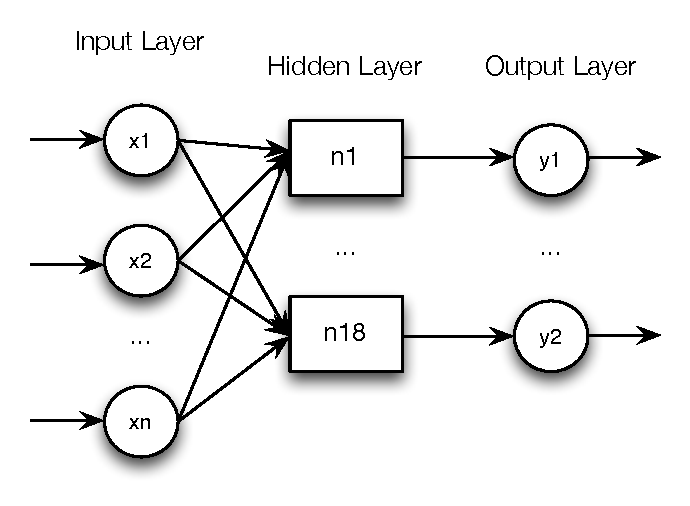
\includegraphics[height=50mm]{lstm/lstm_netz}
\caption{LSTM-Netz}
\label{fig:lstm_netz}
\end{figure}


\subsubsection{Datenaufbereitung}
\label{sec:lstm_data}

In Kapitel \ref{Kapitel 1 TODO} wird beschrieben wie die Daten aufgenommen und
im Allgemeinen verarbeitet werden, bevor sie den Klassifikatoren zur
Verfügung gestellt werden. Diese erhalten jeweils einzelne Frames mit je 64
Daten. Die Daten entprechen dem Frequenzspektrum im Umfeld der
Referenzfrequenz von $18500\text{kHz}$. Eine Geste wurde mit 32 Frames
aufgenommen. Für \ac{LSTM}-Netzwerke sind diese rohen Daten eher ungeignet. Die
Netzwerke können zwar im Allgemeinen mit unverarbeiteteten Daten umgehen,
trotzdem ist ein Vorverarbeitung sinnvoll, da sich dadurch die Verallgemeinerung
des Problems verbessert, die Trainingszeit verkürzt und die benötigten Beispiele
verringern \textbf{Cite}. Aus diesen Gründen wird eine Vorverarbeitung der Daten
vorgenommen. 

Die Beispieldaten sind auf verschiedenen Hardwareplattformen mit
unterschiedlichen Lautstärke und Aufnahmelautstärke Konfigurationen erzeugt
worden. Der Wertebereich dieser Daten ist somit groß und unterschiedlich bei
gleichen Gesten. Das Problem dass durch diese Varianz der Wertemenge entseht
ist, dass \acp{LSTM} Netze (bzw. jede Form von neuronalen Netzen) die Gewichte
entsprechend groß kalibirieren muss, um Unterschiede ausgleichen zu können und
eine verallgemeinertes Ergebnis zu liefern. Da jedoch das (später beschriebene)
Trainigsverfahren iterativ die Gewichte in kleinen Schritten anpasst, führen
große Gewichte zu einem hohen Trainingsaufwand. Um dies zu vermeiden werden die
Daten normalisiert. Konkret wird dabei der Maximalwert eines Frames als
Normierungsfaktor gewählt. Dadurch liegen alle Werte im Intervall $[0,1]$.
Eine Transformation \textbf{richtiges Wort?} des Spektrums hin zu den
Veränderungen der Spektrums im Vergleich zum Ruhespektrum wird ebenfalls
vorgenommen. Dies wird aufgrund durchgeführter Tests vorgenommen, die eine
bessere Klassifizierungen für die transformierten Daten bescheinigen
(\textbf{Tests einbinden}). Der allgemeine Ruhezustand wird aus den Beispielen
des Ruhzustands (Geste 6 und 7) durch das normalisierte Mittel gewonnen. Der
Ruhezustand wird dann von jedem Beispiel abgezogen. Es werden hierbei lediglich
die Beispiele verwendet, denkbar ist jedoch auch die Aufnahme des Ruhezustands
auf dem Zielgerät, um spezifischere Daten zu erhalten. 

Bei der Betrachtung der Daten fällt auf, dass der Doppler-Effekt in einem
kleinen Intervall um die Referenzfrequenz auftritt und die Daten außerhalb
dieses Intervalls keine große Bedeutung spielen. Aus diesem Grund ist eine
Verkleinerung der Frame Größe in Betracht zu ziehen. Da jedoch eine manuelle
Betrachtung aller Daten nicht möglich ist, lässt sich diese Beobachtung nicht
manuell verifzieren. Daher werden mehrere \ac{LSTM}-Netze mit unterschiedlichen
Inputframelängen trainiert und die Ergebnisse verglichen. \textbf{TODO Tabelle
mit Ergebnissen} Erstaunlicherweise ist die aufgestellte Vermutung falsch und die
Netzwerke ohne zugeschnittenen Trainingsdaten klassifizieren besser. 
\begin{table*}
\centering
\begin{tabular}{|c|c|c|c|c|c|c|c|}
\hline
 Fold 		& Cut & Peephole & Neurons & 250 & 500 & 750 & 1000 \\
 \multirow{12}{*}{1}&\multirow{4}{*}{0}&\multirow{2}{*}{true}&16&28,39\%&27,30\%&26,54\%&27,19\%\\
  & & &18&29,14\%&28,06\%&26,00\%&26,89\%\\
  & &\multirow{2}{*}{false}&16&30,55\%&29,58\%&26,44\%&26,76\%\\
  & & &18&26,65\%&26,22\%&25,35\%&24,81\%\\
  &\multirow{4}{*}{16}&\multirow{2}{*}{true}&16&36,73\%&35,21\%&33,37\%&32,61\%\\
  & & &18&33,69\%&31,20\%&29,90\%&29,47\%\\
  & &\multirow{2}{*}{false}&16&30,44\%&30,44\%&29,36\%&29,79\%\\
  & & &18&30,34\%&27,95\%&27,95\%&28,17\%\\
  &\multirow{4}{*}{24}&\multirow{2}{*}{true}&16&33,59\%&32,07\%&31,53\%&32,07\%\\
  & & &18&35,75\%&33,69\%&29,04\%&27,74\%\\
  & &\multirow{2}{*}{false}&16&33,15\%&33,15\%&32,39\%&32,18\%\\
  & & &18&32,50\%&31,20\%&30,01\%&29,79\%\\
  \multirow{12}{*}{2}&\multirow{4}{*}{0}&\multirow{2}{*}{true}&16&35,54\%&31,96\%&31,74\%&31,64\%\\
  & & &18&33,59\%&31,64\%&29,36\%&29,58\%\\
  & &\multirow{2}{*}{false}&16&34,99\%&32,07\%&30,34\%&29,58\%\\
  & & &18&36,94\%&33,91\%&31,96\%&32,18\%\\
  &\multirow{4}{*}{16}&\multirow{2}{*}{true}&16&33,69\%&32,74\%&30,01\%&29,98\%\\
  & & &18&33,26\%&31,74\%&30,01\%&29,69\%\\
  & &\multirow{2}{*}{false}&16&32,50\%&30,66\%&28,49\%&27,63\%\\
  & & &18&35,64\%&35,10\%&31,85\%&31,09\%\\
  &\multirow{4}{*}{24}&\multirow{2}{*}{true}&16&35,97\%&34,56\%&34,45\%&33,48\%\\
  & & &18&33,26\%&32,72\%&29,58\%&33,48\%\\
  & &\multirow{2}{*}{false}&16&35,32\%&34,74\%&32,61\%&32,29\%\\
  & & &18&31,85\%&30,99\%&30,34\%&28,71\%\\
\hline
\end{tabular}
\caption{Datentests LSTM-Netz}
\label{tab:inputtests}
\end{table*}
Eine weitere Beobachtung die gemacht werden kann ist, dass benachbarte
Datenpunkte sich nicht wesentlich unterscheiden. Dies kann genutzt werden um die
Eingabedimension zu verringern, indem z.B. jeweils zwei benachbarte Datenpunkte
miteinander addiert werden. Dies kann auch mit dem verkleinern der Frames
kombiniert werden. Um den Einfluss auf das Klassifierzungsverhalten von
\ac{LSTM}-Netzen zu zeigen sind auch hier Tests durchgeführt worden.
\textbf{TODO Tabelle mit Ergebnissen} Das Ergebnis zeigt, dass die Netze ohne
die Summe benachbarter Werte besser klassifizieren als mit der Summe. 

Weitere Methoden der Datenvorverarbeitung wurden ebenfalls untersucht, jedoch
hat dies die Ergebnisse ebenfalls negativ beeinflusst, weshalb sie nicht näher
betrachtet wurden. Darunter fällt u.a. die statische Eliminierung von Rauschen.
Diese Methode setzt jeden Wert der unter einem bestimmten Schwellwert ist zu 0,
da dies kein signifikanter Beitrag zur Geste ist sondern ein Rauschen. Das
Ergebnis dieser Untersuchung ist jedoch unbefridigend, sodass die Idee nicht
genutzt wird. \textbf{TODO Messwerte?}
 


\subsubsection{Anpassung des Klassifikators}
\subsubsection{Implementierung}
Da es zum Ende des Projektes ein Programm geben soll, indem alle Klassifikatoren 
eingebunden sind, haben sich alle Teilnehmer auf ein Interface geeingtt, was 
jeder Klassifikator implementieren muss. Dies ist die abstrakte Klasse \textit{IClassifier}.

\textbf{TODO Klassendiagramm}

Die Implementation des \ac{LSTM}-Klassifikators ist in der Klasse LSTM zu finden.
Für diese wurde \cite{PyBrain} verwendet. Diese Bibliothek stellt verschiedene
Machine Learning Algorithmen bereit, unter anderem Neuronale Netzwerke mit 
\ac{LSTM}-Neuronen.
Außerdem wurden in der Datei \texttt{util.py} verschiedene Hilfsfunktionen
erstellt.
Des weiteren werden Konfigurationseinstellungen in einer Datei gespeichert und zur 
initialisierung der geladen. 
Da beabsichtigt ist mit dem Programm den PC zu steuern, wurde die Python Bibliothek 
\cite{Python-uinput} eingebunden. Mit dieser können Keycodes an den Kernel geschickt werden.
Die Bibliothek funktioniert nur unter Linux und erfordert Root-Rechte.
Im folgenden wird auf die Implementation der einzelnen MEthoden der 
\textit{IClassifier}-Klasse eingegangen.

\subsubsection*{Live Klassifikation}
Für die Live Klassifikation wurde zwei verschiedene Ideen implementiert. 
Bei beiden wird zuerst die \textit{classify} Methode der LSTM-Klasse 
aufgerufen. Diese bekommt den Datensatz der aktuellen Aufnahme übergeben. 
Der Datensatz enthält ein Array mit 64-Datenpunkten. Die übergebenen Daten werden 
Normalisiert und anschließend wird der Durchschnitt abgezogen, wie in Kapitel 
\autoref{sec:lstm_data} beschrieben. Nachdem die Daten vorbearbeitet wurden, 
werden diese einer \textit{classify1}-Methode übergeben. 
\begin{lstlisting}[language=Python,caption={Classify
Variante 1},label={lst:lstm_classify1}]{lst:lstm_classify1}
def __classify1(self,data):
	self.datalist.append(data)
	self.datanum += 1
	if(self.datanum % 32 == 0):
		self.net.reset()
		out = self._activateSequence(self.datalist)
		print(str(out))
		self.datalist = []
		self.datanum = 0
		return out
	return -1
\end{lstlisting}

Die Methode \textit{classify1} speichert so lange die übergebenen Datenwerte, 
bis 32-Werte aufgenommen wurden. Diese 32-Werten werden dem \ac{LSTM}-Netz 
übergeben und eine Klassifikation gestartet. Da es bei diesem Ansatz passieren kann, 
dass eine Geste nicht komplett in diesen 32-Werte enthalten ist, wurde ein zweite 
Idee umgesetzt, welche in der Methode \textit{classify2} umgesetzt ist.

\begin{lstlisting}[language=Python,caption={Classify
Variante 2},label={lst:lstm_classify2}]{lst:lstm_classify2}
def __classify2(self, data):
	self.datanum += 1
	self.datalist.append(data)
	if(self.datanum % 32 == 0):
		self.has32 = True
	if(self.has32):
		self.net.reset()
		Y_pred = self._activateSequence(self.datalist)
		del self.datalist[0]
		self.predHistory[0] = Y_pred
		self.predHistory = np.roll(self.predHistory, -1)
		expected = stats.mode(self.predHistory, 0)
		if(expected[1][0] >= self.predHistHalfUpper):
			if(int(expected[0][0]) != self.previouspredict):
				oldPrevious, oldPredCounter = self.previouspredict, self.previouspredict
				self.previouspredict = int(expected[0][0])
				self.predcounter = 1
				return oldPrevious, oldPredCounter
			else:
				self.predcounter += 1
				if(self.predcounter == 4):
					print(str(self.previouspredict))
					self.outkeys.outForClass(self.previouspredict)
				return self.previouspredict, self.predcounter
	return -1, -1
\end{lstlisting}

Die Methode \textit{classify2} speichert so lange die übergebenen Datenwerte, 
bis 32-Werte aufgenommen wurden. Diese 32-Werten werden dem \ac{LSTM}-Netz 
übergeben und eine Klassifikation gestartet. Die erkannte Geste wird in einer 
Liste gespeichert. Von dieser Liste wird, mittels der Python-Funktion mode, 
der Wert ermittelt der am häufigsten vorkommt. Ist dieser Wert größer als eine 
definierte Schranke wird er in \textit{previouspredict} gespeichert. Wenn vier 
mal hinter einander die gleiche Geste erkannt wurde, wird diese ausgegeben.

\subsubsection{Training}
Für das Trainieren von Neuronalen Netzen bietet PyBrain verschiedene 
Trainer an:
\begin{itemize}
\item BackpropTrainer
\item RPropMinusTrainer
\end{itemize}
Da der RPropMinusTrainer eine Erweiterung des BackpropTrainer ist, wurde mit 
diesem trainiert. Für die verwendung der zu verfügung gestellten Trainer 
muss ein PyBrain Dataset erstellt werden. Um dieses zu erstellen wurde eine 
Methode geschrieben. Diese erstellt aus den Aufnahmen ein Dataset. Dazu wird 
aus den Aufnahmen ein Array generiert. Nach der generierung werden die Daten 
normalisiert. Anschließend werden noch weitere Schritte durchgeführt, diese 
sind in Kapitel \autoref{sec:lstm_data} beschrieben und können mit den folgenden 
Parametern konfiguriert werden:
\begin{itemize}
\item \textbf{merge67} Dieser Parameter gibt an, ob die Gesten 6 und 7 
zusammengefasst werden sollen.
\item \textbf{average} Definiert ob nach der Normalisierung der Datensätze der 
Durchschnitt abgezogen wird. 
\item \textbf{cut} Gibt an um wieviel jeder Datensatz beschnitten wird.
\item \textbf{fold} Konfiguriert ob jeder der Datensätze verwendet wird oder
wieviele übersprungen werden.
\end{itemize} 
Nach der Erstelung des Datasets wird es gespaltet. Für das Training werden 
80\% und für die Validierung 20\% verwendet.

Für die Validierung des Netzes wurde eine Methode implementiert, die anahnd 
des Testsets validiert wie gut das Neuronale Netzwerk die Gesten erkennt. Nach 
diesem Test wird eine Matrix erstellt, die die Anzahl der richtig erkannten Gesten 
sowie die Anzahl der falsch erkannten Gesten anzeigt. 

\textbf{TODO MAtrix anzeigen}

\subsubsection{Evaluation}
Für die Evaluation der Netzwerke ein Testparcour entwickelt. In diesem wird 
jede der 6 Gesten 10 mal durchgeführt und die Anzahl der Erfolge protokolliert. 
Dies wurde wurde für jede Klassifikations-Idee durchlaufen. In Tabelle 
\cite{tab:eval} sind die Ergebnisse festgehalten.
\begin{table}
\begin{tabular}{|c|c|c|c|c|c|c|c|}
\hline
 Geste 		& 1 & 2 & 3 & 4 & 5 & 6 & 7 \\
 \hline
 classify1  &	&	&	&	&	&	&	\\
 \hline
 classify2  &	&	&	&	&	&	&	\\
\hline
\end{tabular}
\caption{Evaluation LSTM-Netz}
\label{tab:eval}
\end{table}

Nach den Tests fällt auf das Geste 1, .. sehr gut erkannt werden. Geste .. ..
jedoch nciht so gut.
\subsection{Fazit}
- LSTM (NN) können Eingaben nur synchron verarbeiten und nicht asynchron wie ein
Gehrin
- zusätzliche Einflüsse wie Botenstoffe die sich auf die Neuronenaktivität
auswirken werden ebenfalls nicht nachgebildet. 

\nocite{schaul2010,GERS2001,WIKI2013,Schmidhuber2013,LSTM1,Nerbonne1}
